\documentclass[aspectratio=169]{beamer}

\usetheme{Madrid}
\usecolortheme{default}
\usepackage{graphicx}
\usepackage{booktabs}

\graphicspath{{./}{../screenshots/}}

\title{Breast Cancer Classification using ANN}
\subtitle{B.Tech AI Mini Project}
\author{Student Name}
\institute{Department of Artificial Intelligence}
\date{\today}

\begin{document}

\begin{frame}
  \titlepage
\end{frame}

\begin{frame}{Outline}
  \tableofcontents
\end{frame}

\section{Introduction}
\begin{frame}{Problem Statement}
  \begin{itemize}
    \item Classify breast tumors as \textbf{Malignant (0)} or \textbf{Benign (1)}
    \item Use a simple Artificial Neural Network (ANN)
    \item Dataset: Breast Cancer Wisconsin (569 samples, 30 features)
    \item Tools: Python, TensorFlow/Keras, scikit-learn
  \end{itemize}
\end{frame}

\section{Dataset}
\begin{frame}{Dataset Overview}
  \begin{center}
    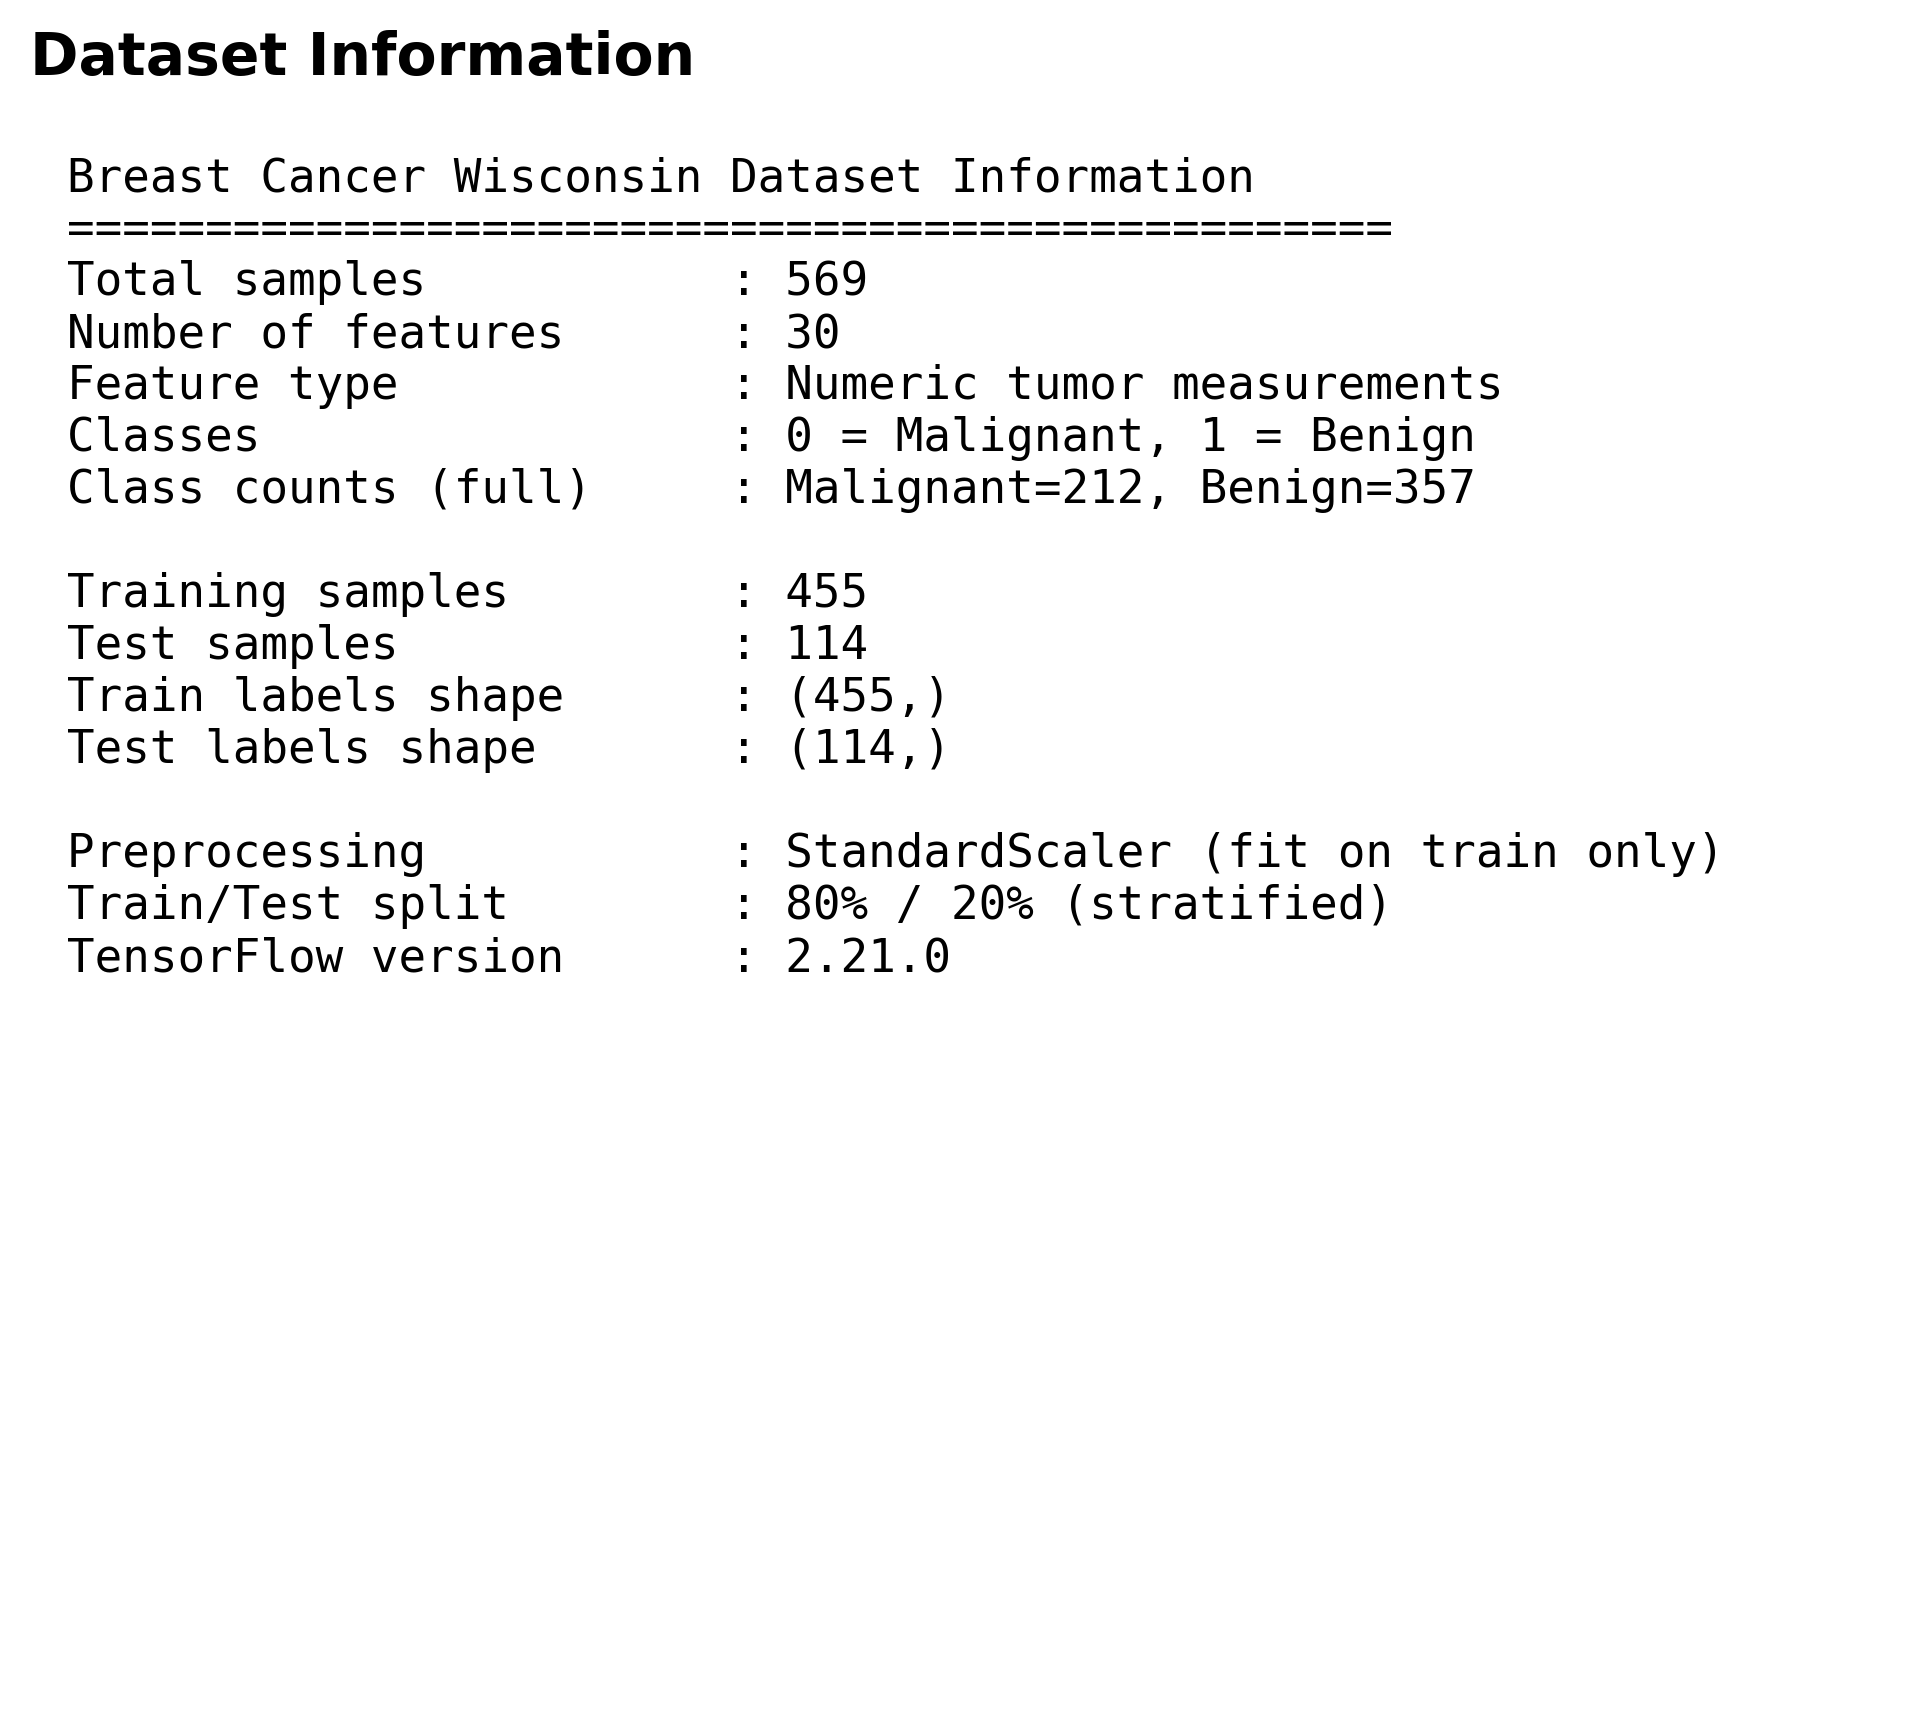
\includegraphics[width=0.92\textwidth,height=0.72\textheight,keepaspectratio]{01_dataset_info.png}
  \end{center}
\end{frame}

\begin{frame}{Class Distribution}
  \begin{center}
    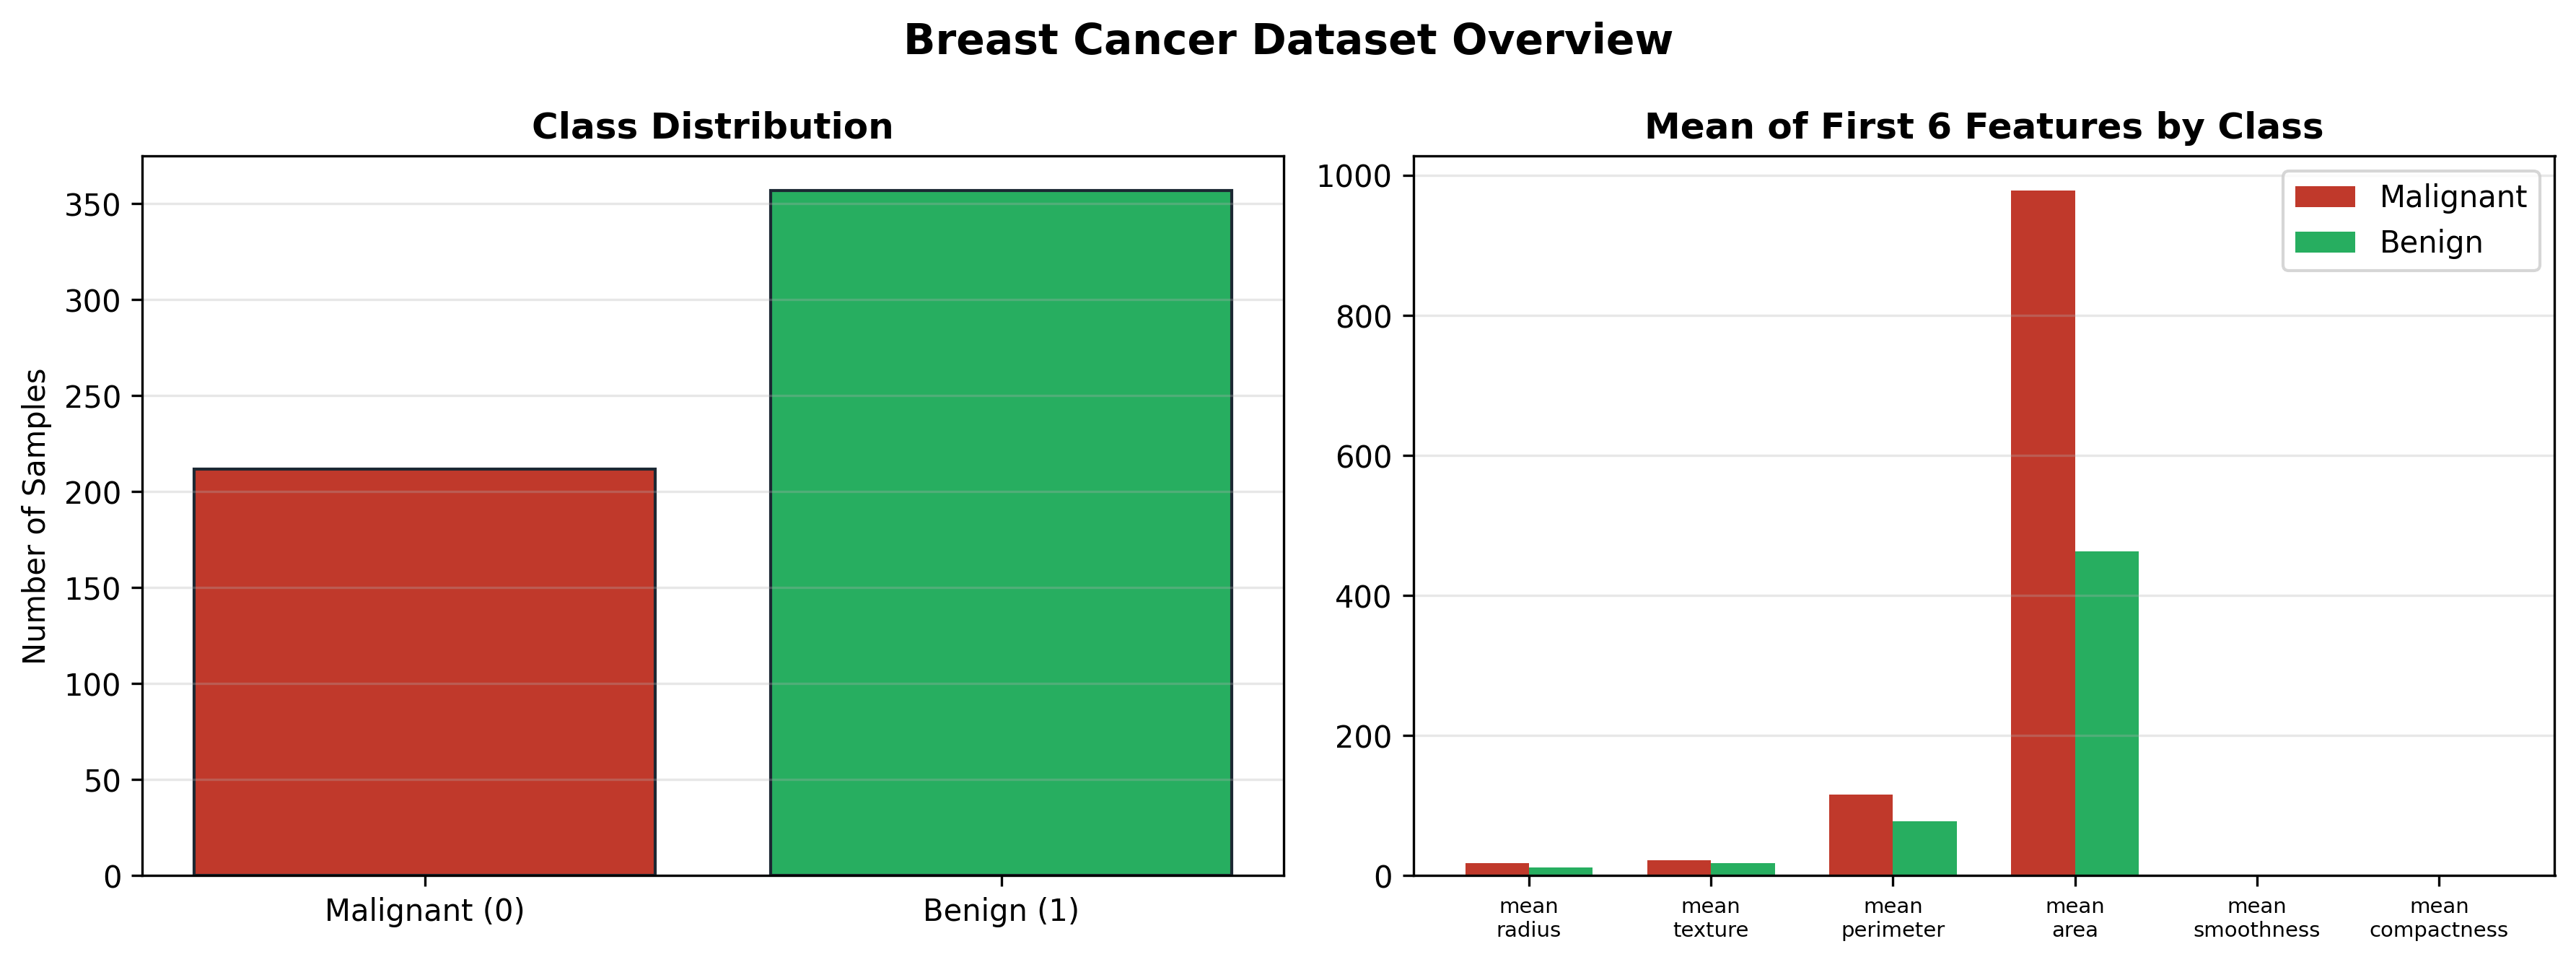
\includegraphics[width=0.92\textwidth,height=0.72\textheight,keepaspectratio]{02_dataset_overview.png}
  \end{center}
\end{frame}

\section{Model}
\begin{frame}{ANN Architecture}
  \begin{center}
    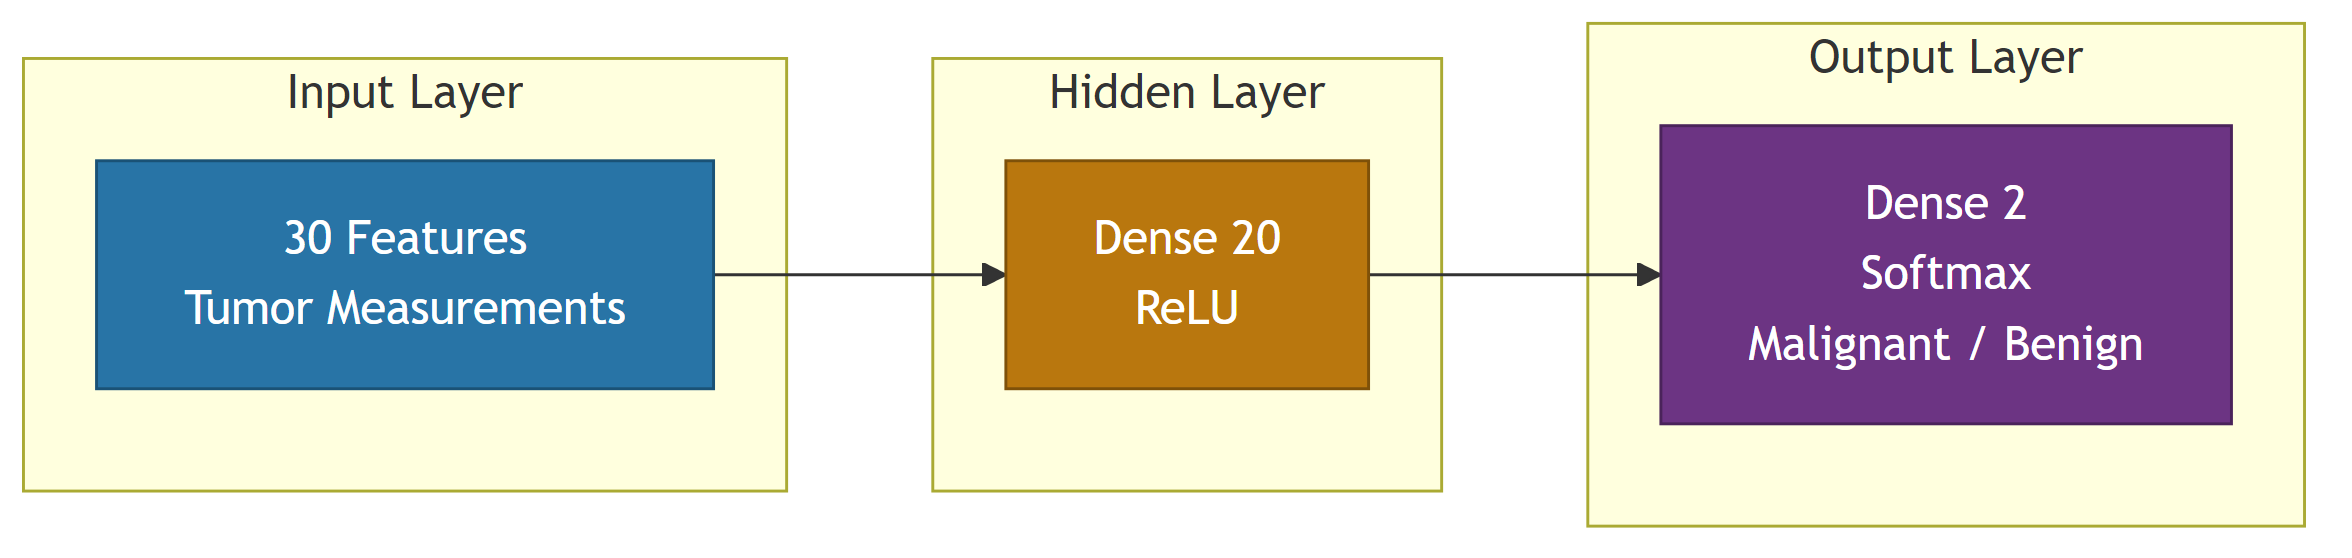
\includegraphics[width=0.9\textwidth,height=0.7\textheight,keepaspectratio]{12_architecture.png}
  \end{center}
\end{frame}

\begin{frame}{Model Summary}
  \begin{center}
    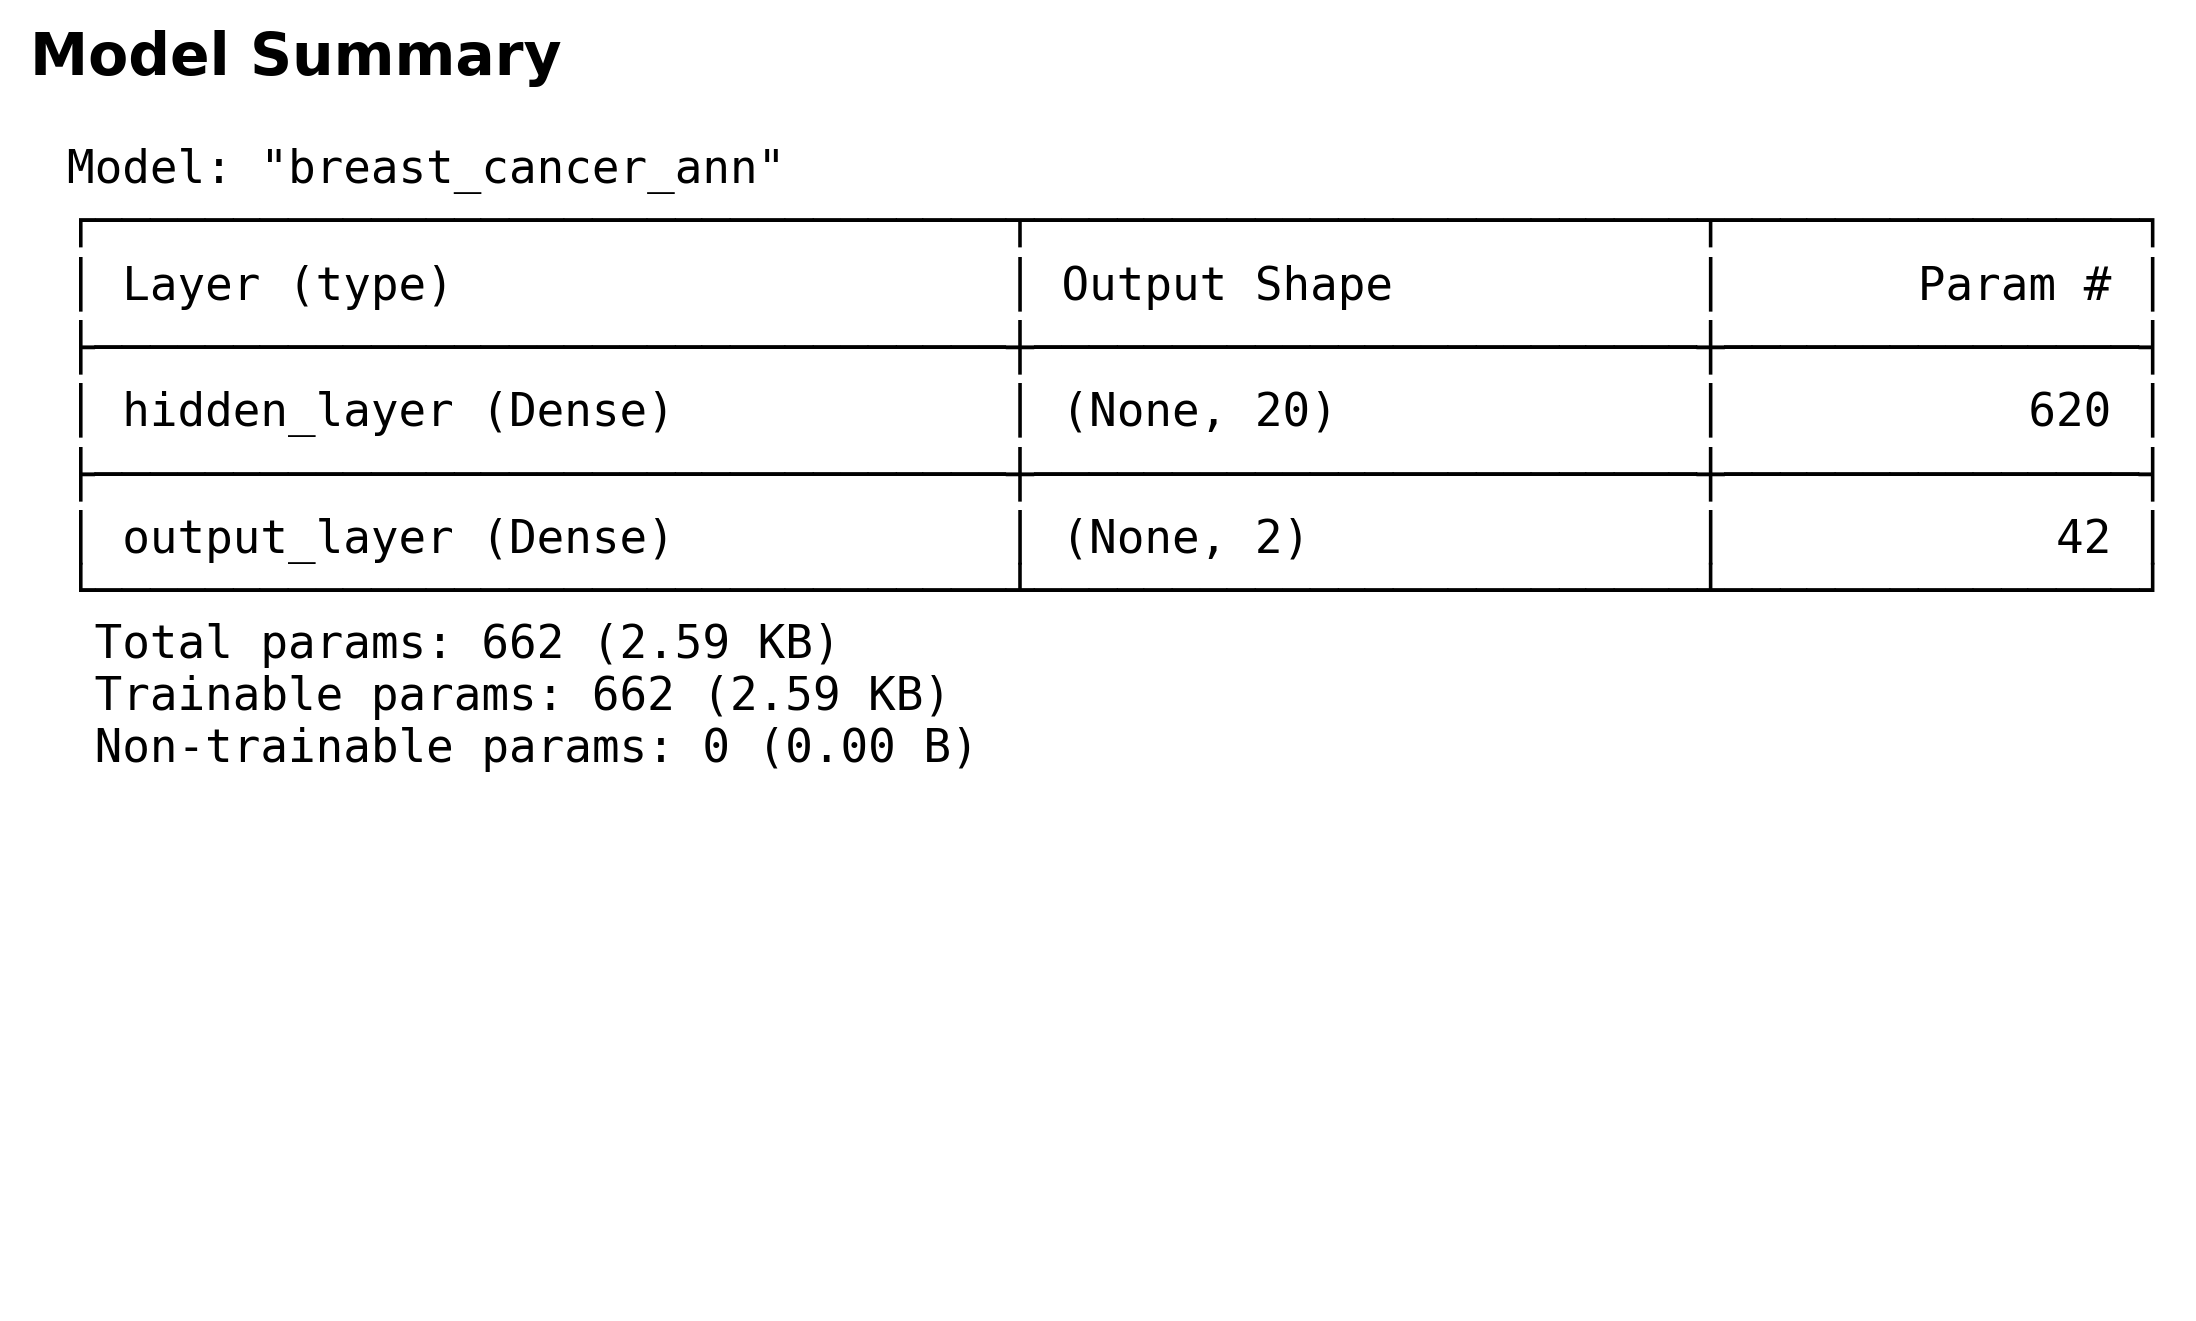
\includegraphics[width=0.85\textwidth,height=0.7\textheight,keepaspectratio]{03_model_summary.png}
  \end{center}
\end{frame}

\section{Training}
\begin{frame}{Training Progress}
  \begin{center}
    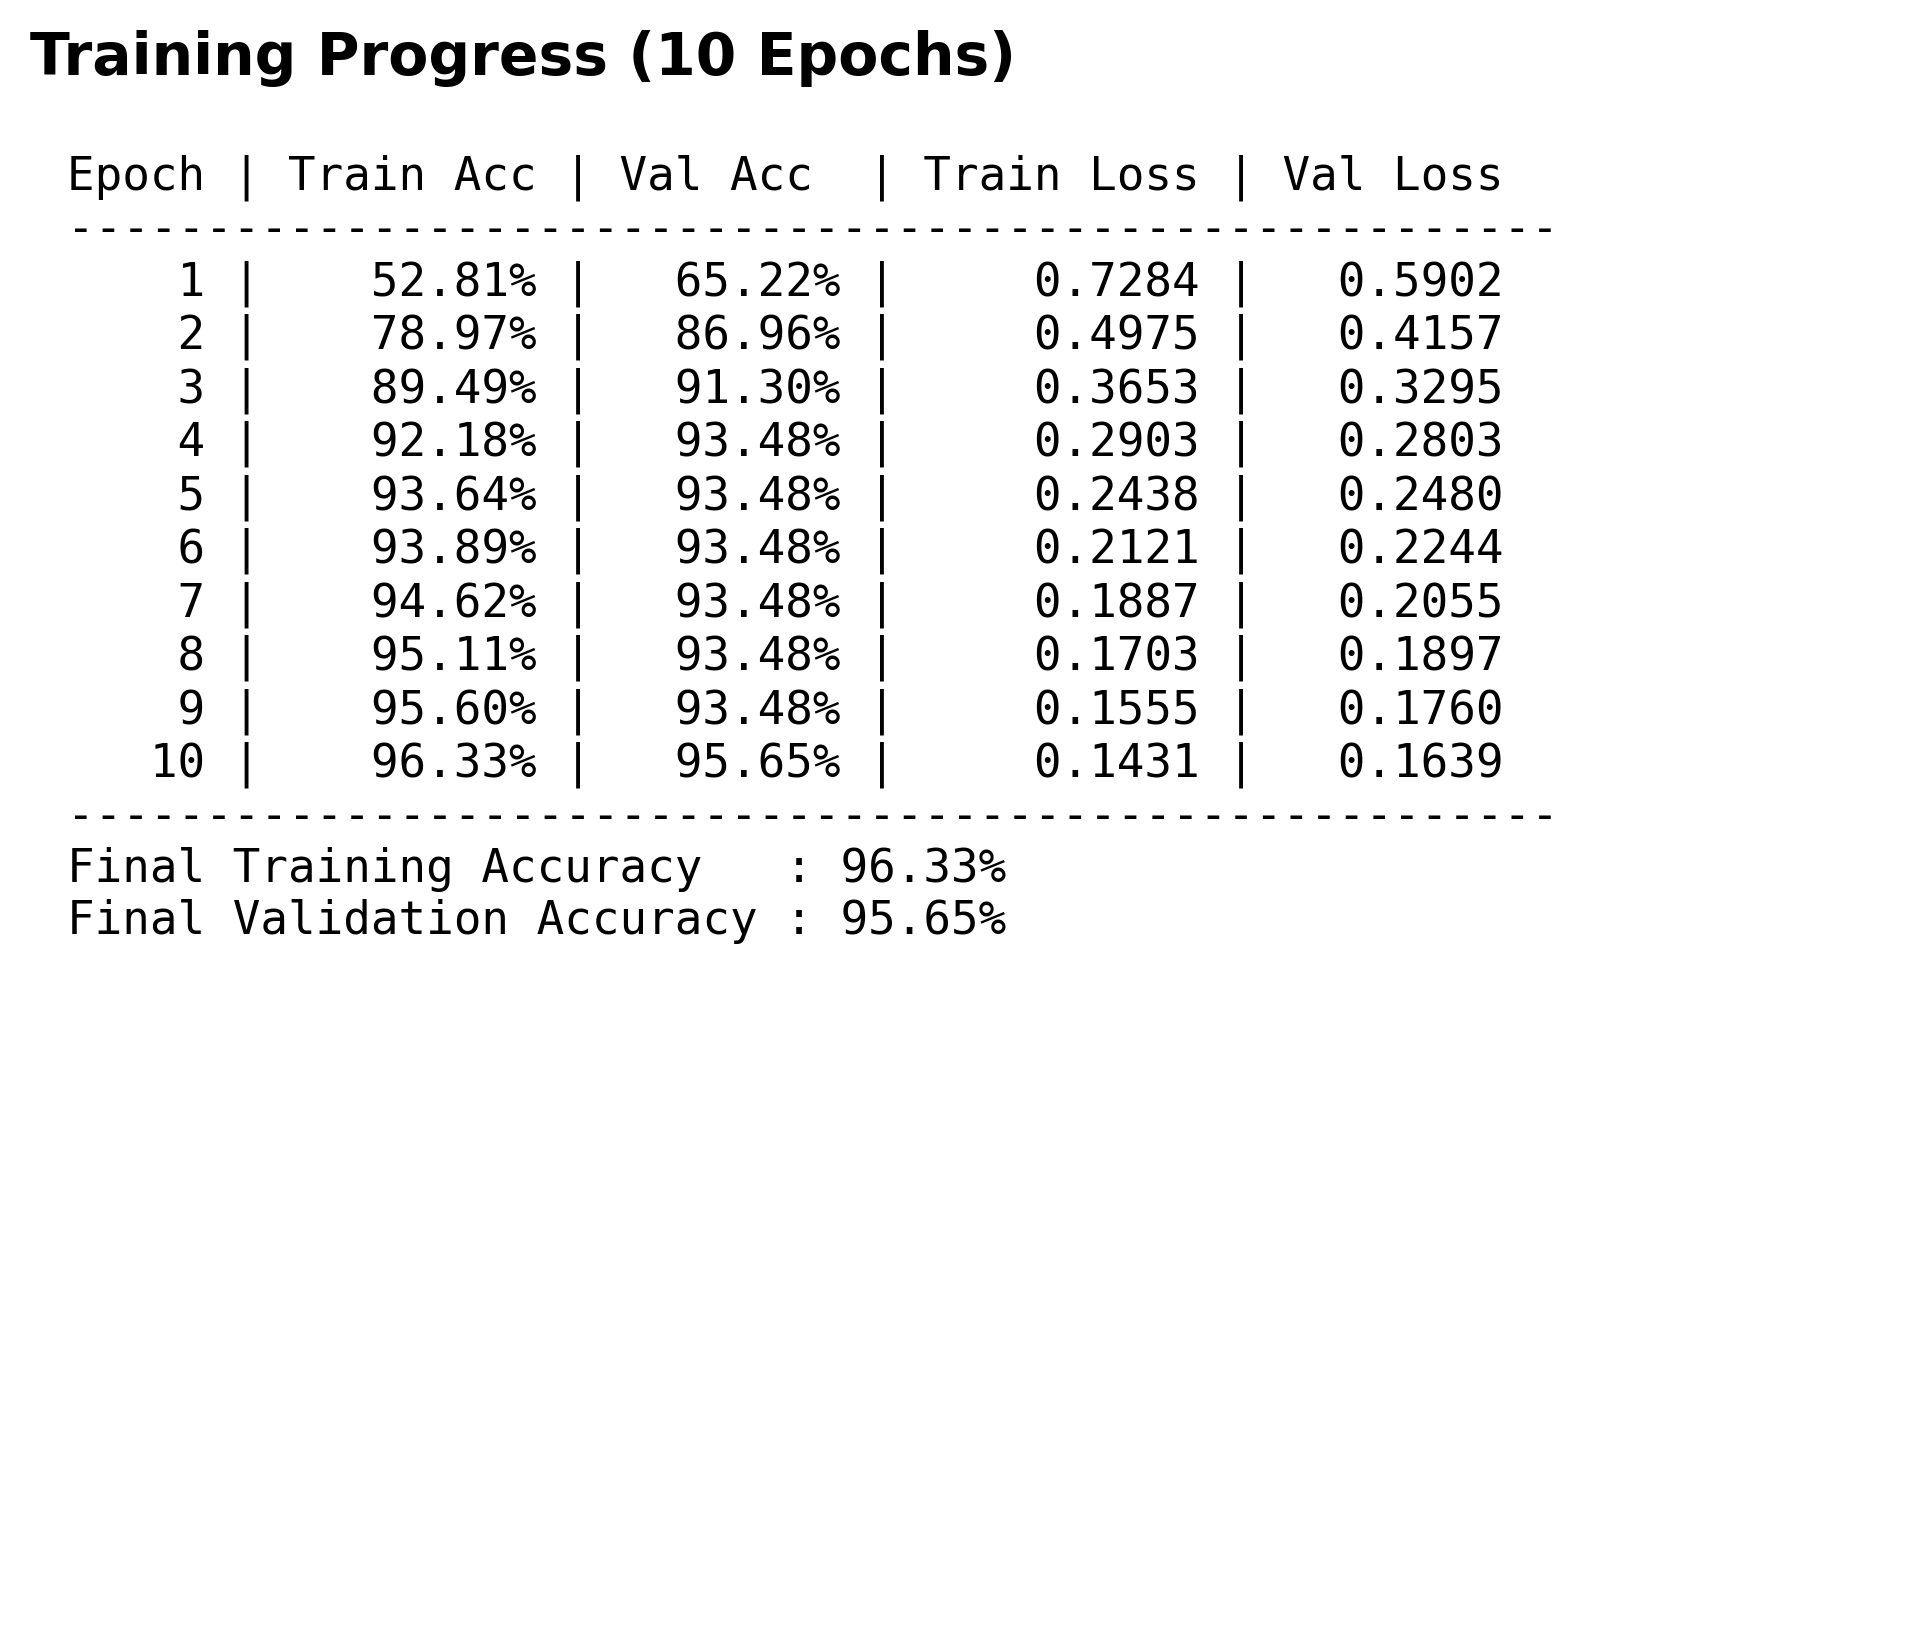
\includegraphics[width=0.9\textwidth,height=0.7\textheight,keepaspectratio]{04_training_progress.png}
  \end{center}
\end{frame}

\begin{frame}{Accuracy Curve}
  \begin{center}
    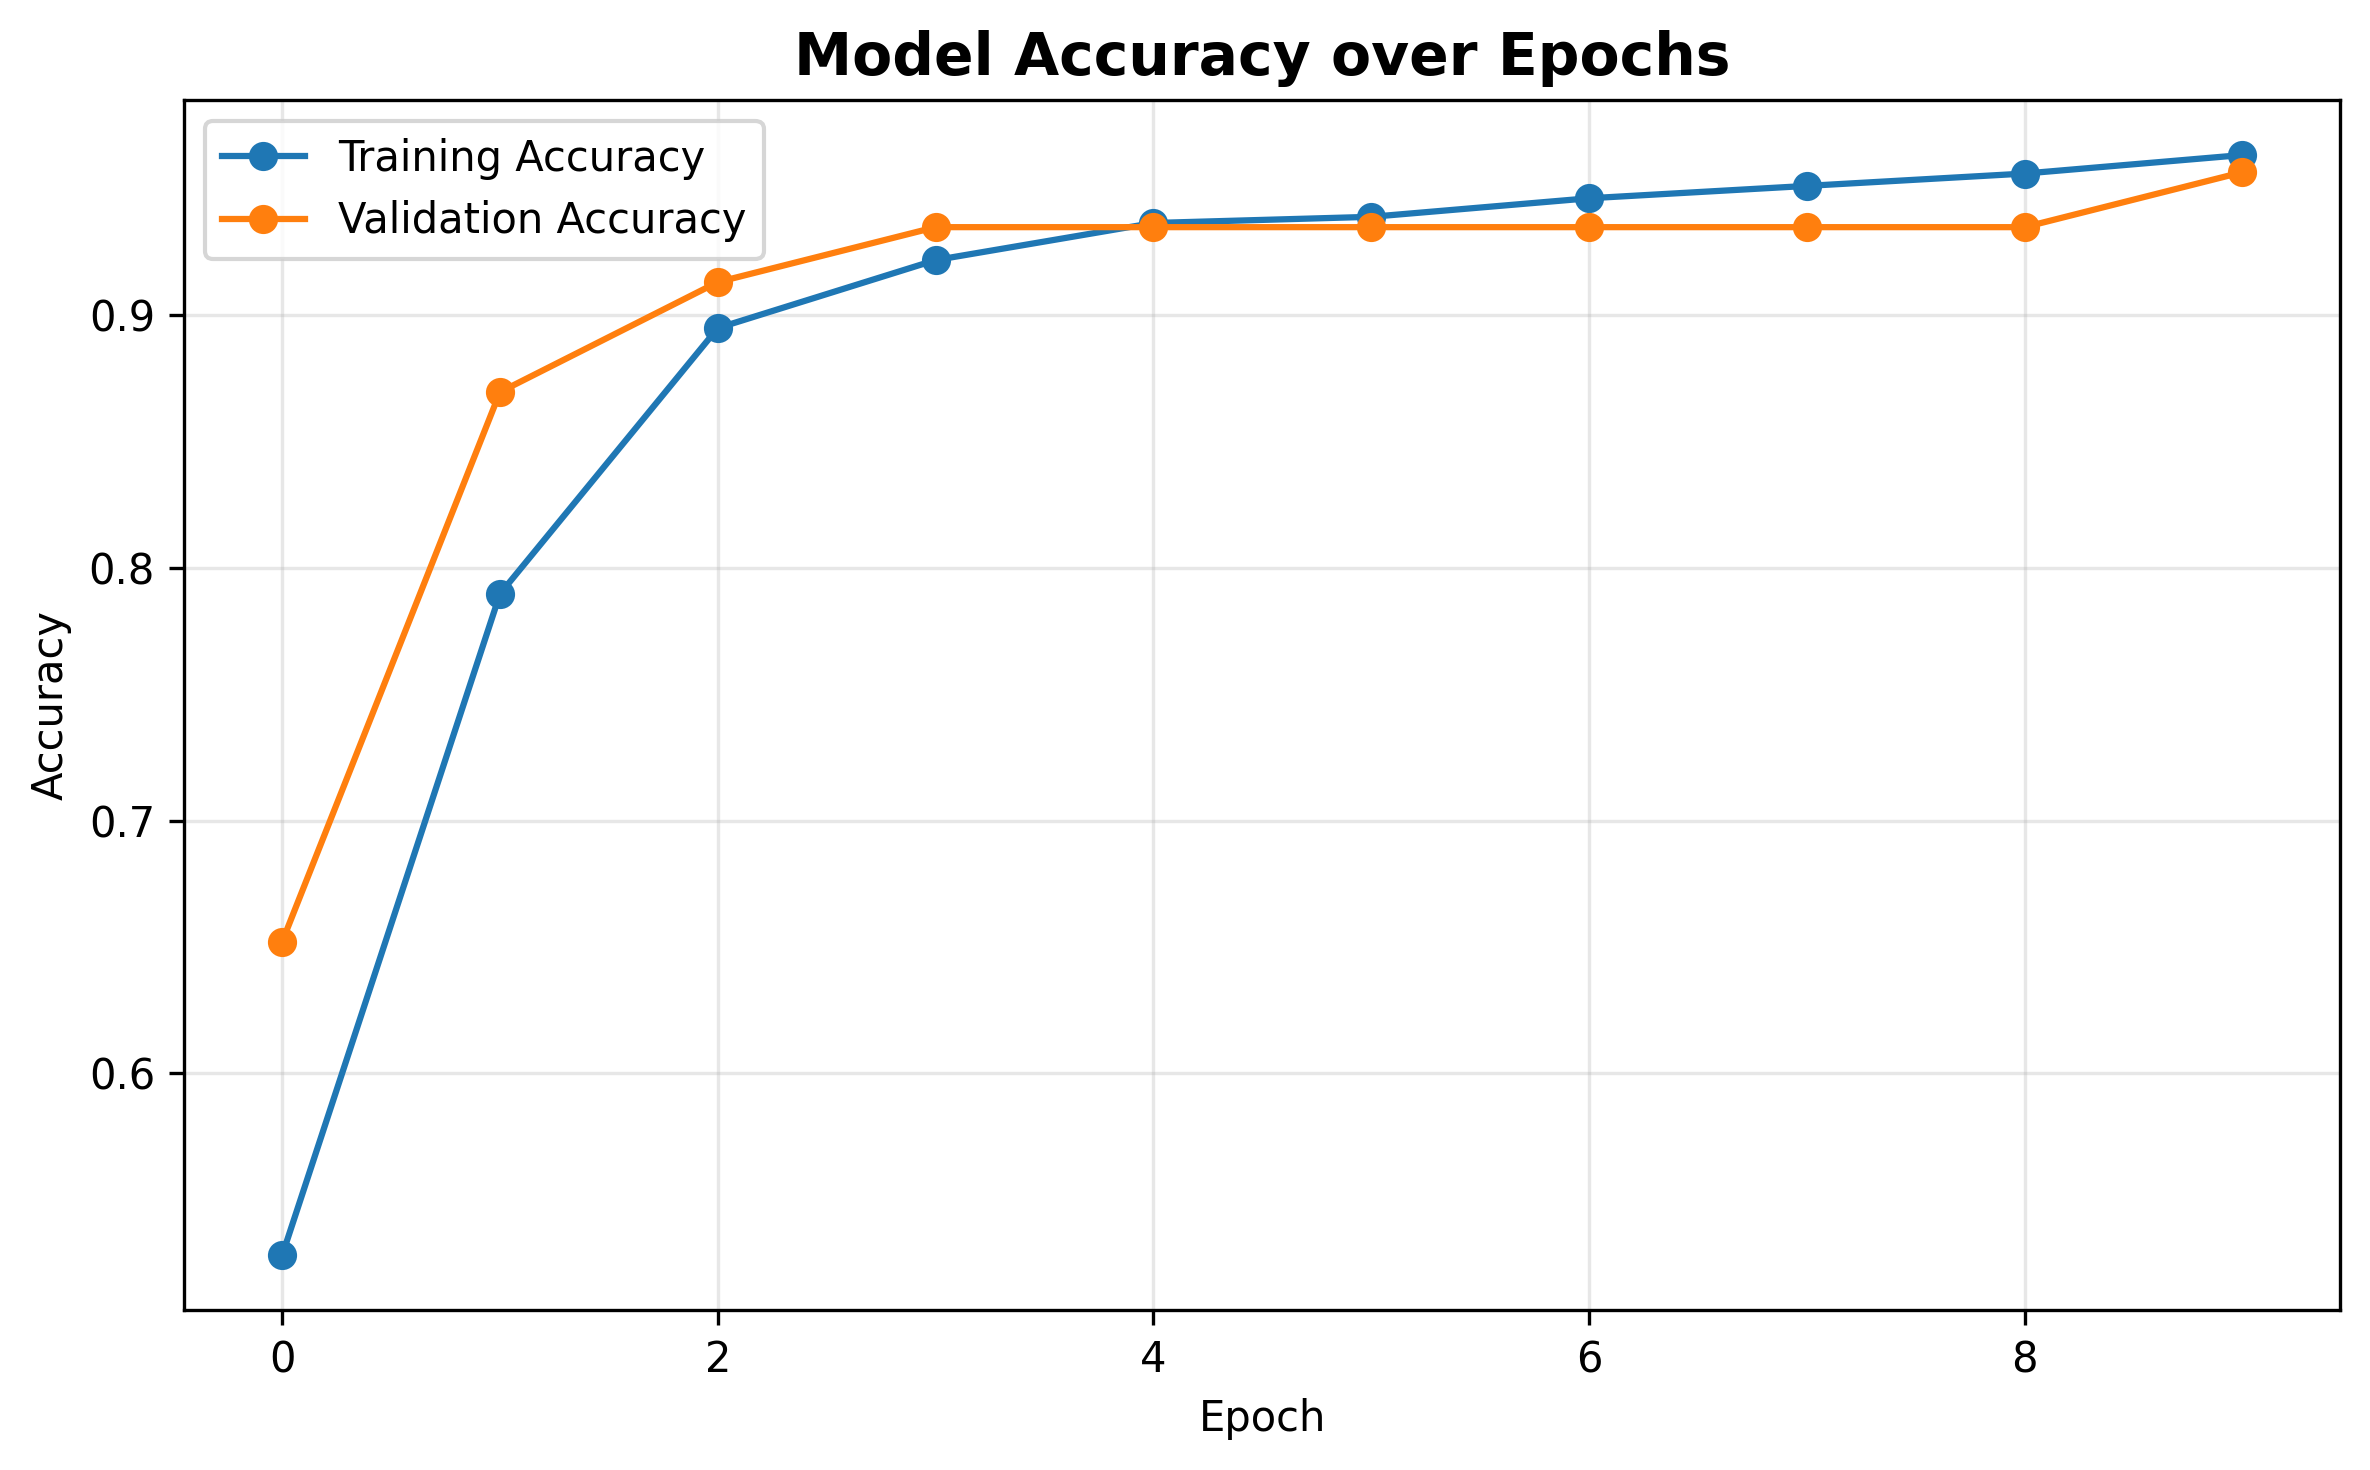
\includegraphics[width=0.85\textwidth,height=0.7\textheight,keepaspectratio]{05_accuracy_curve.png}
  \end{center}
\end{frame}

\begin{frame}{Loss Curve}
  \begin{center}
    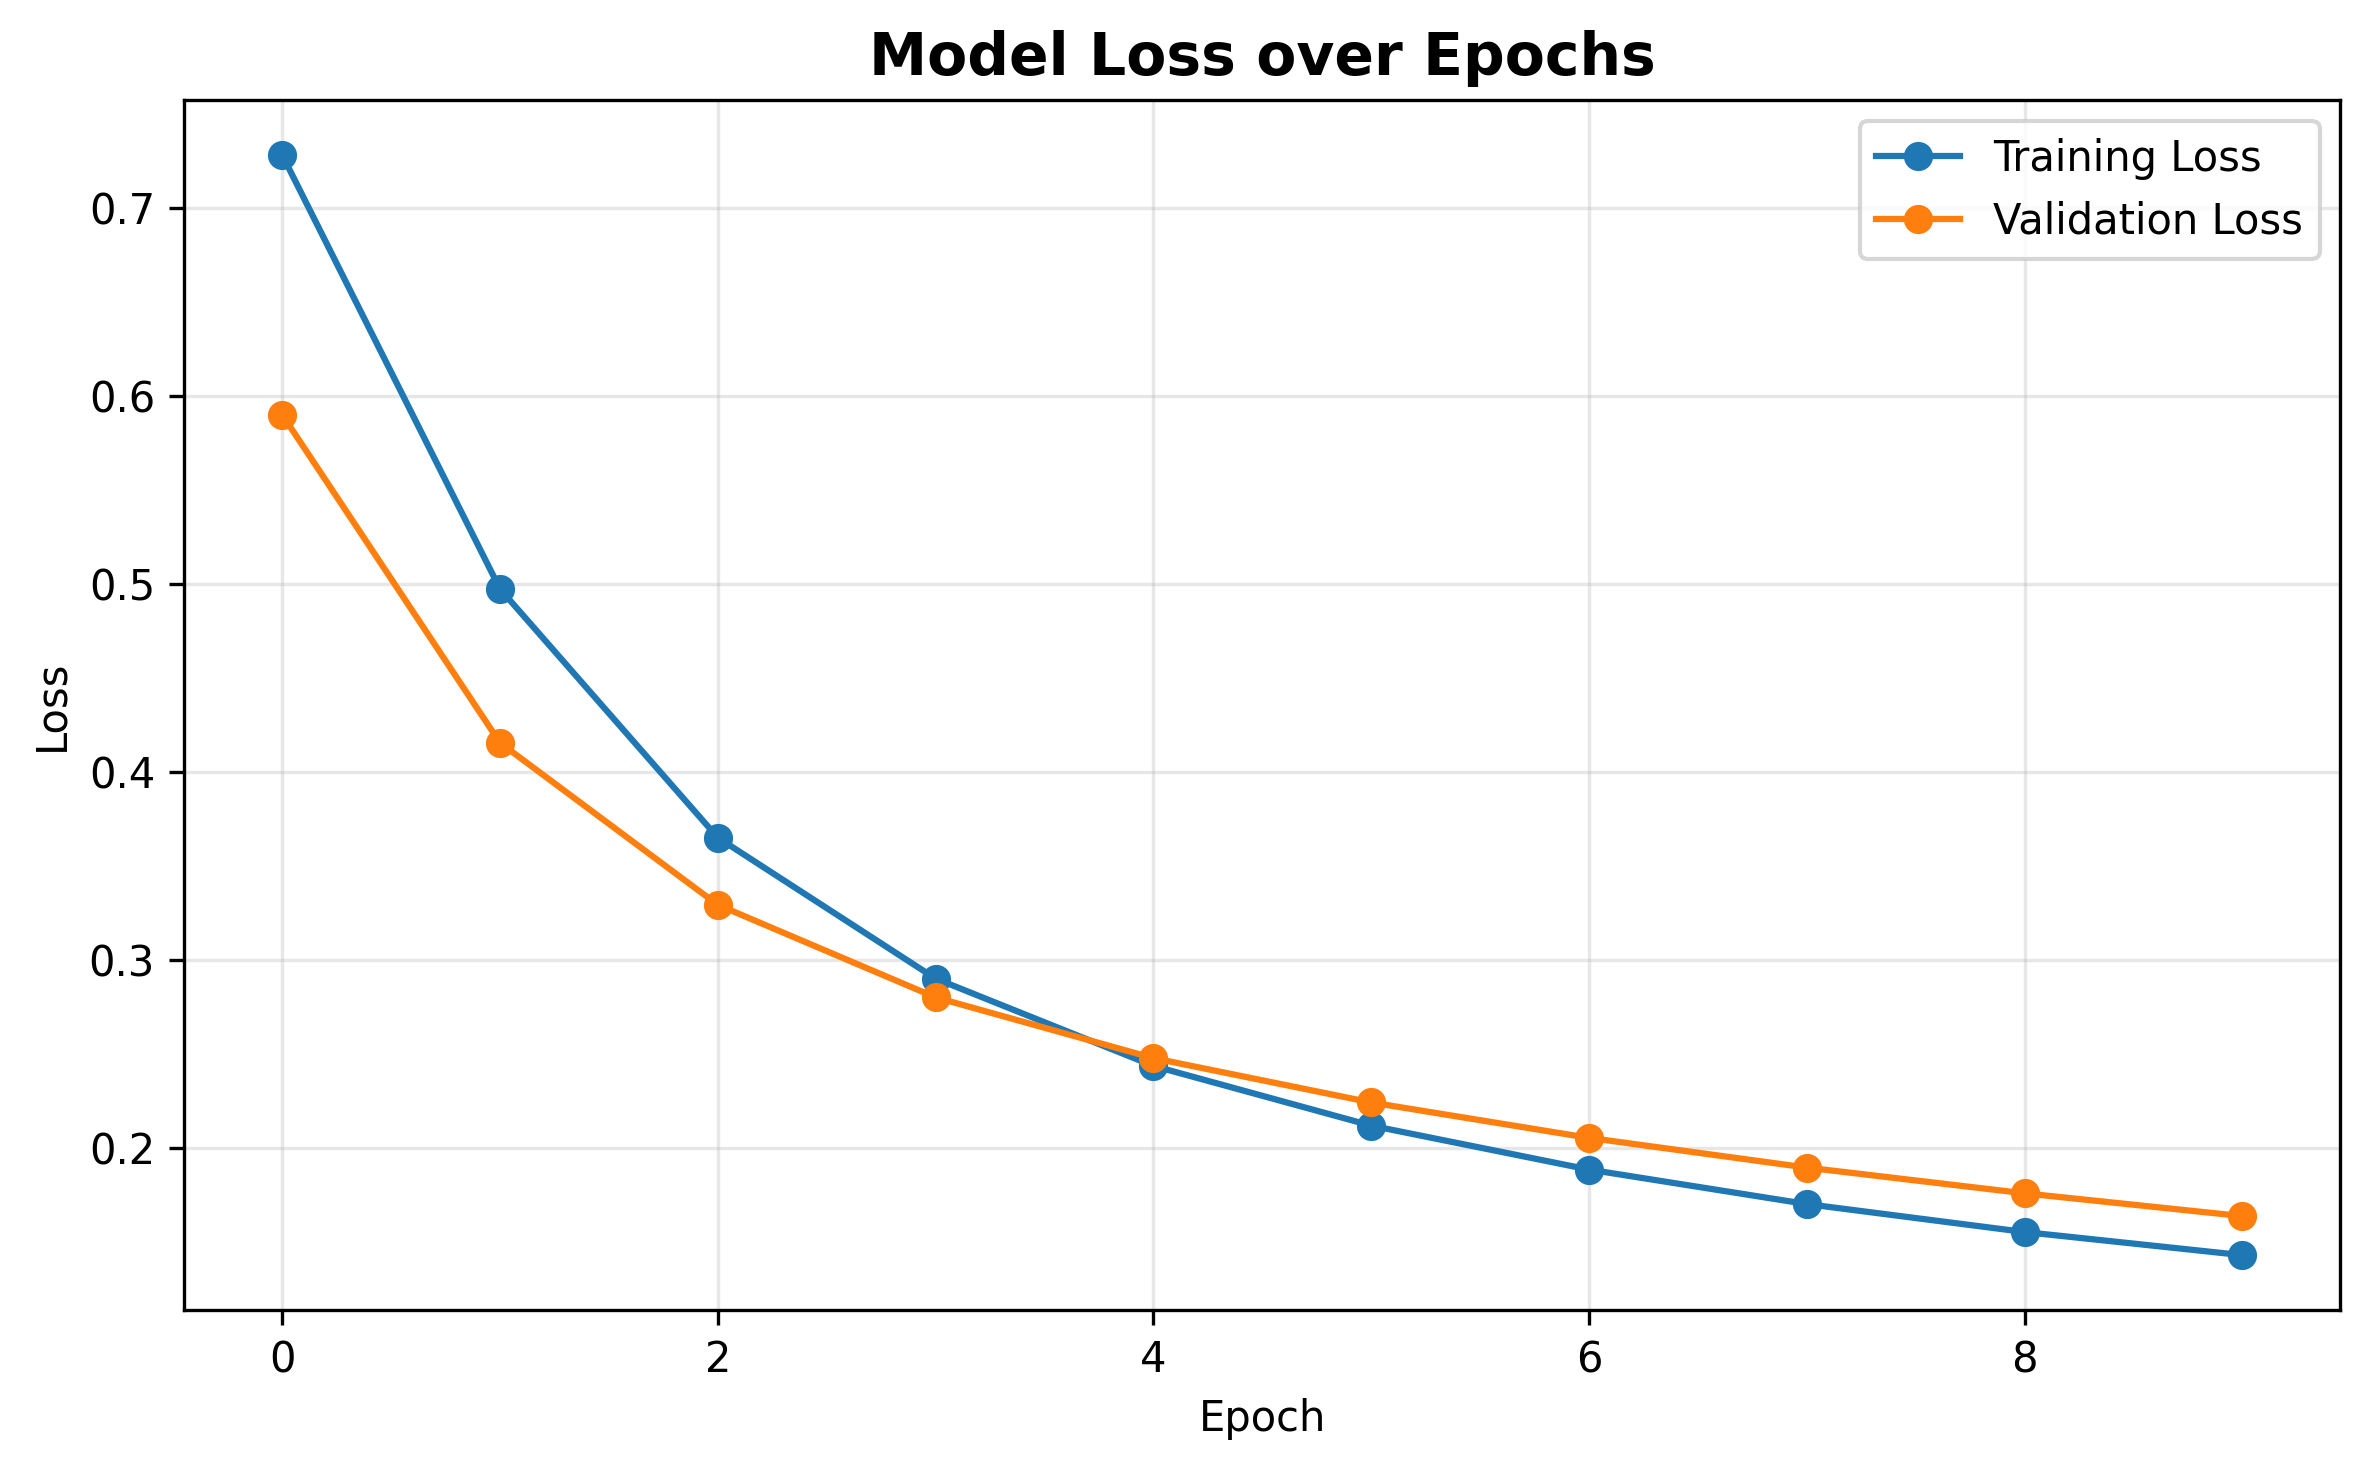
\includegraphics[width=0.85\textwidth,height=0.7\textheight,keepaspectratio]{06_loss_curve.png}
  \end{center}
\end{frame}

\section{Results}
\begin{frame}{Test Accuracy}
  \begin{center}
    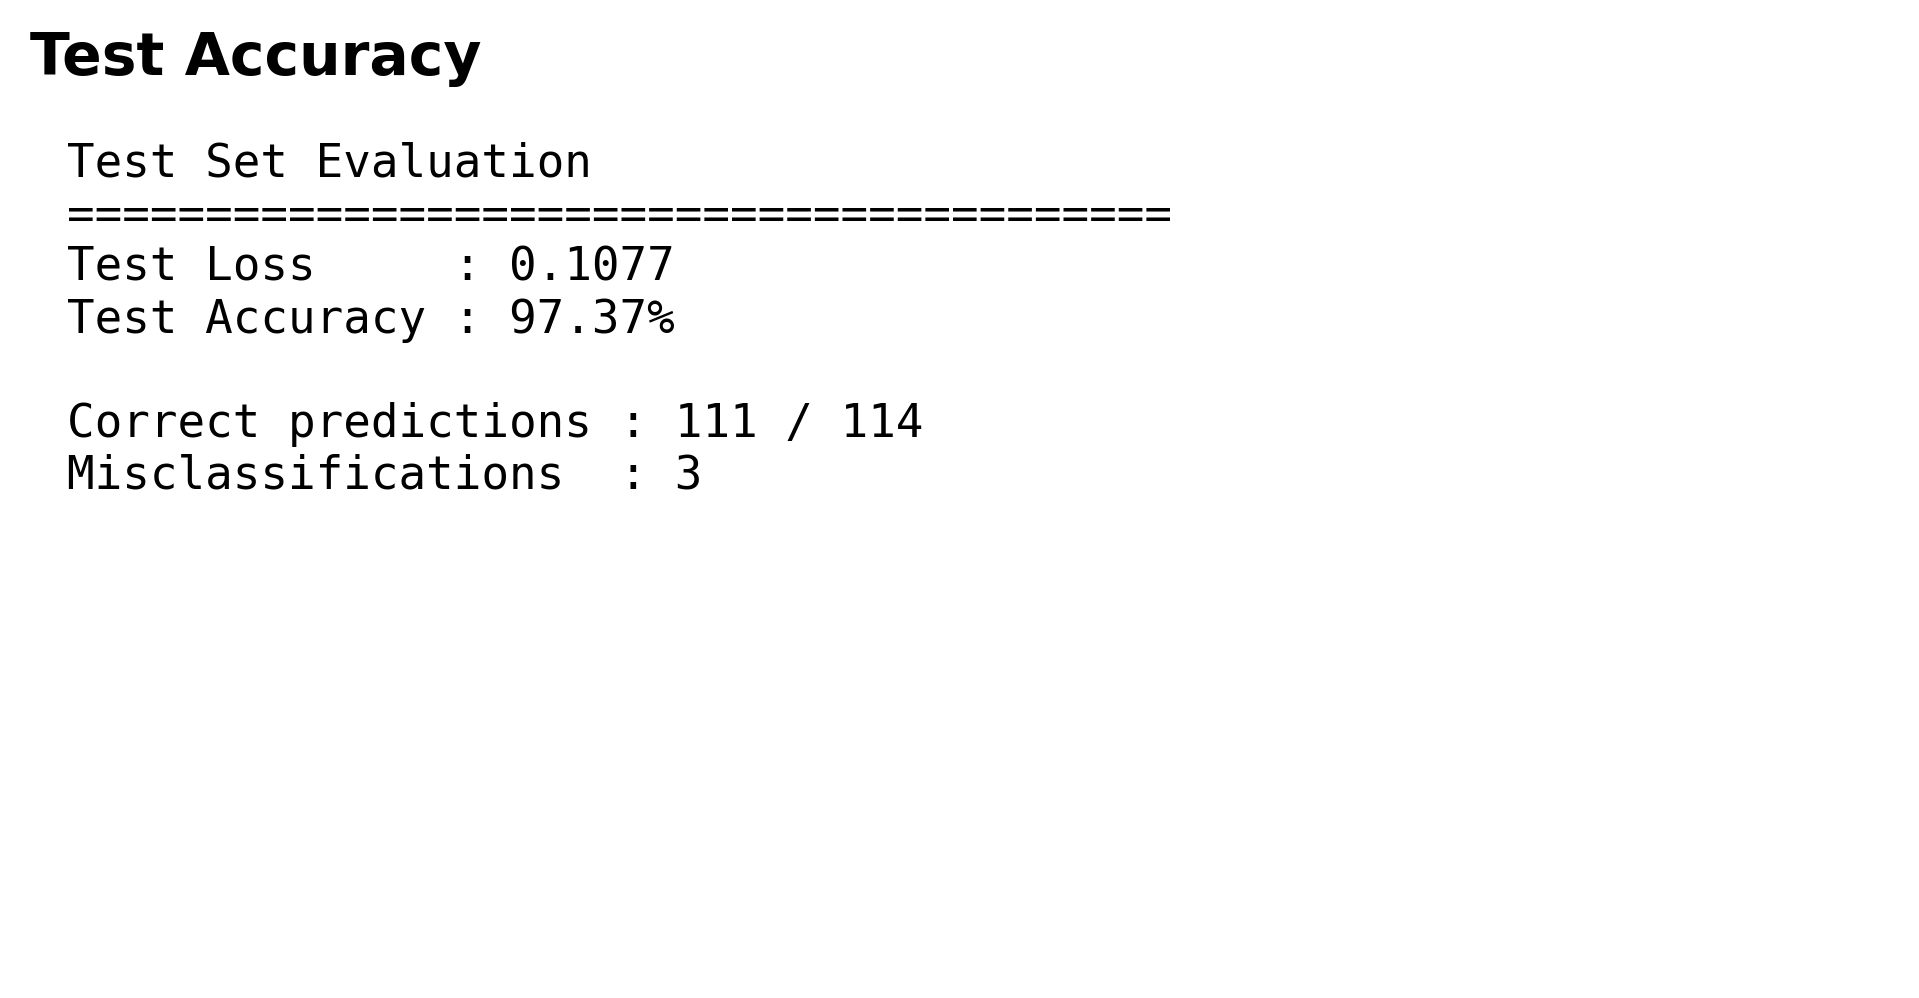
\includegraphics[width=0.8\textwidth,height=0.7\textheight,keepaspectratio]{07_test_accuracy.png}
  \end{center}
\end{frame}

\begin{frame}{Confusion Matrix}
  \begin{center}
    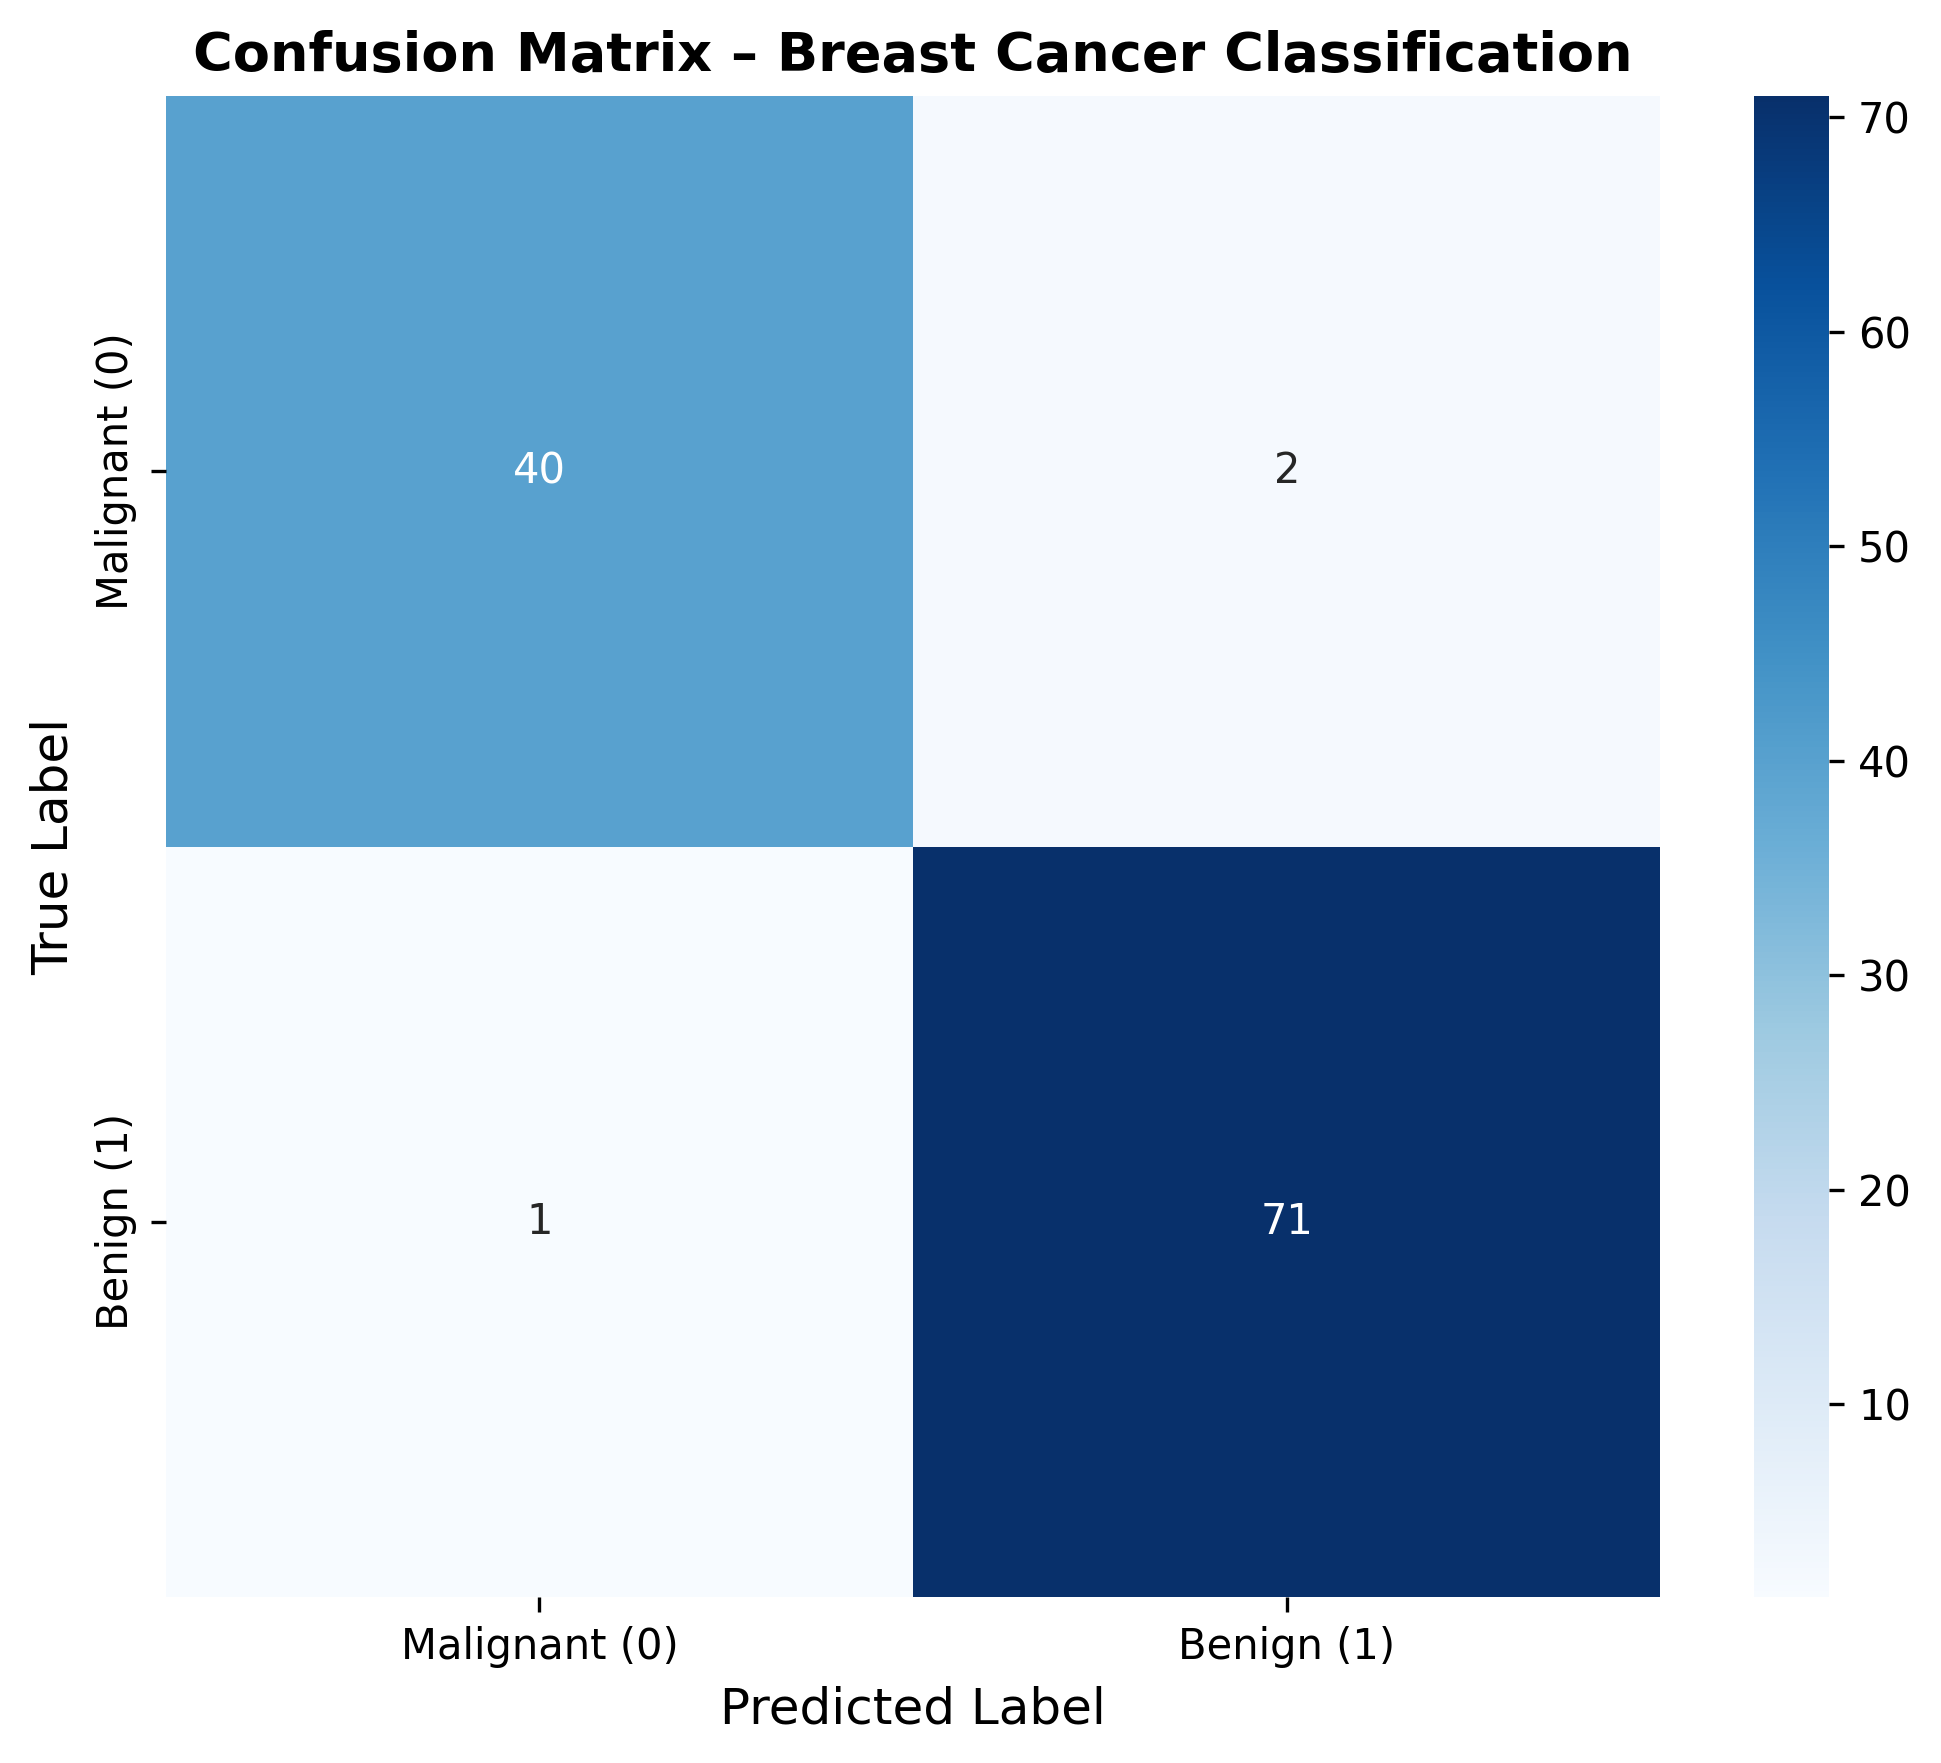
\includegraphics[width=0.65\textwidth,height=0.7\textheight,keepaspectratio]{08_confusion_matrix.png}
  \end{center}
\end{frame}

\begin{frame}{Classification Report}
  \begin{center}
    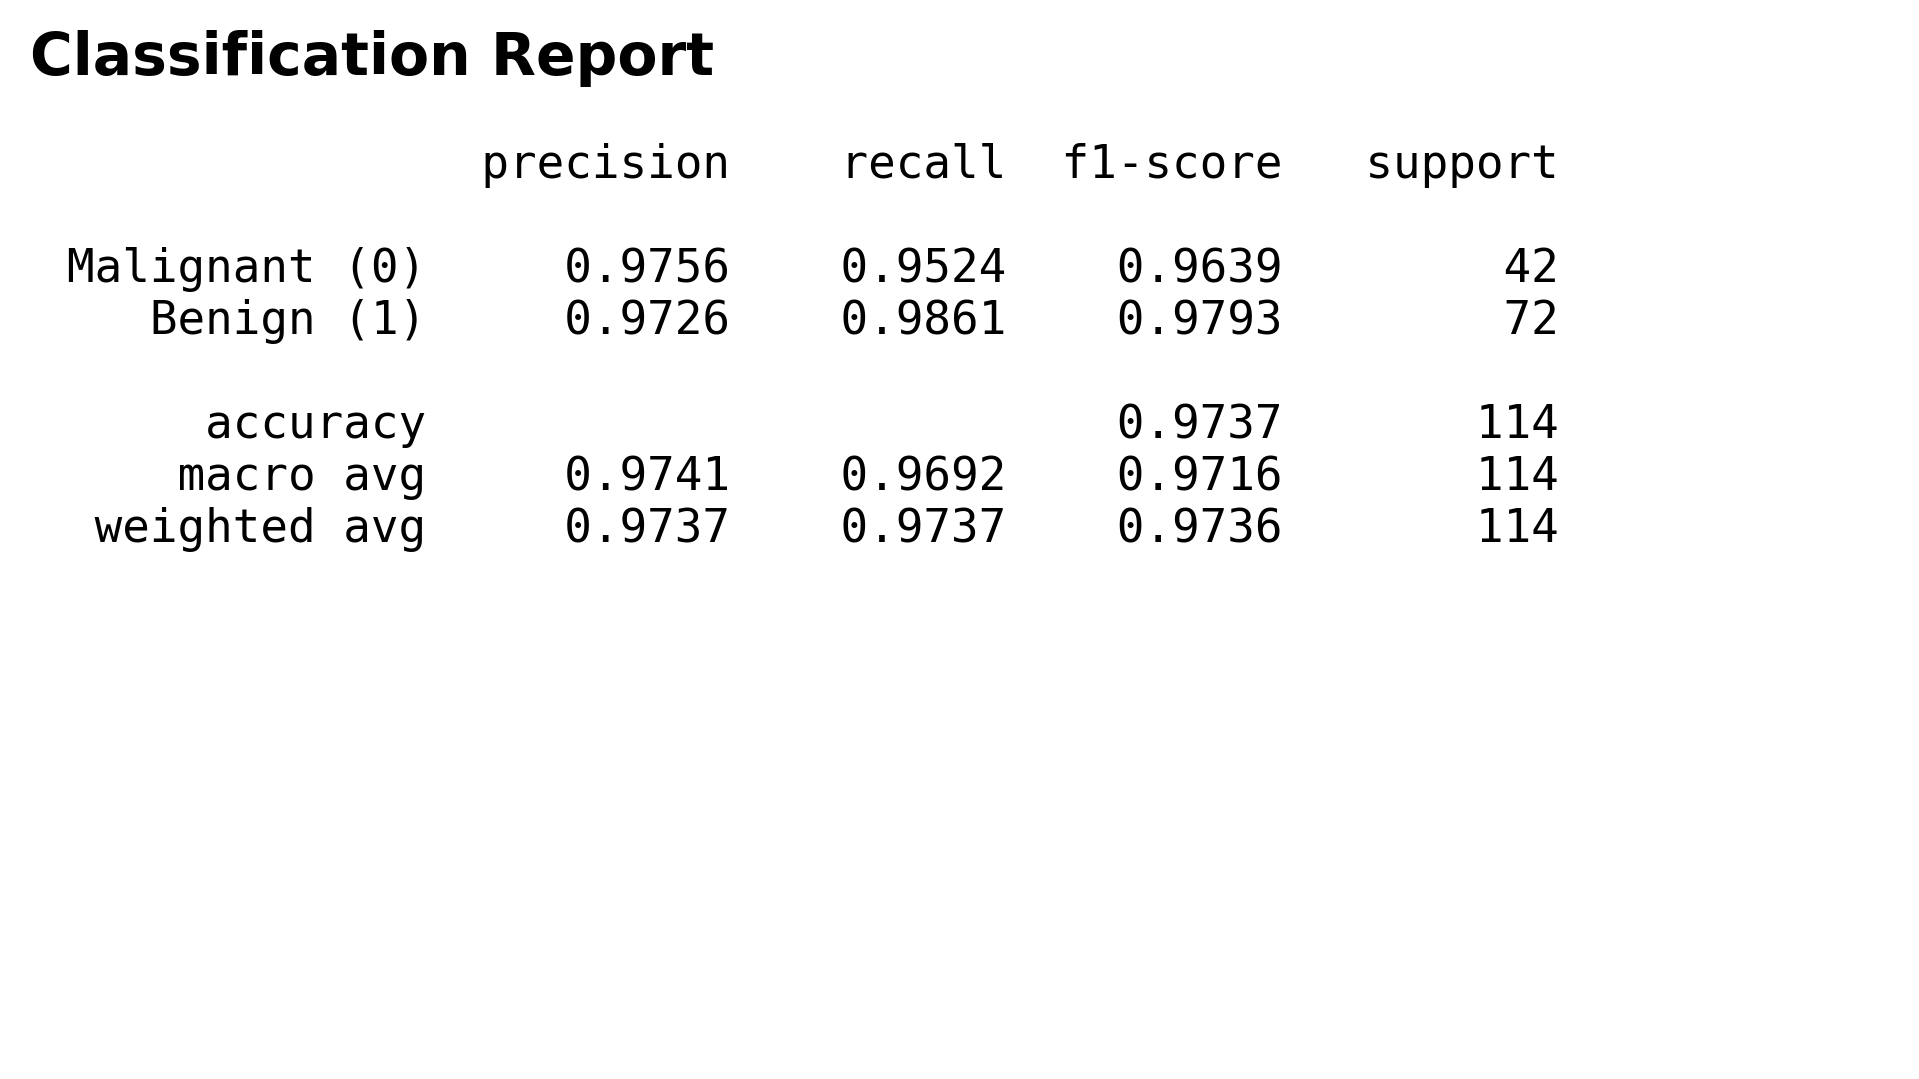
\includegraphics[width=0.9\textwidth,height=0.7\textheight,keepaspectratio]{09_classification_report.png}
  \end{center}
\end{frame}

\begin{frame}{Prediction Demo}
  \begin{center}
    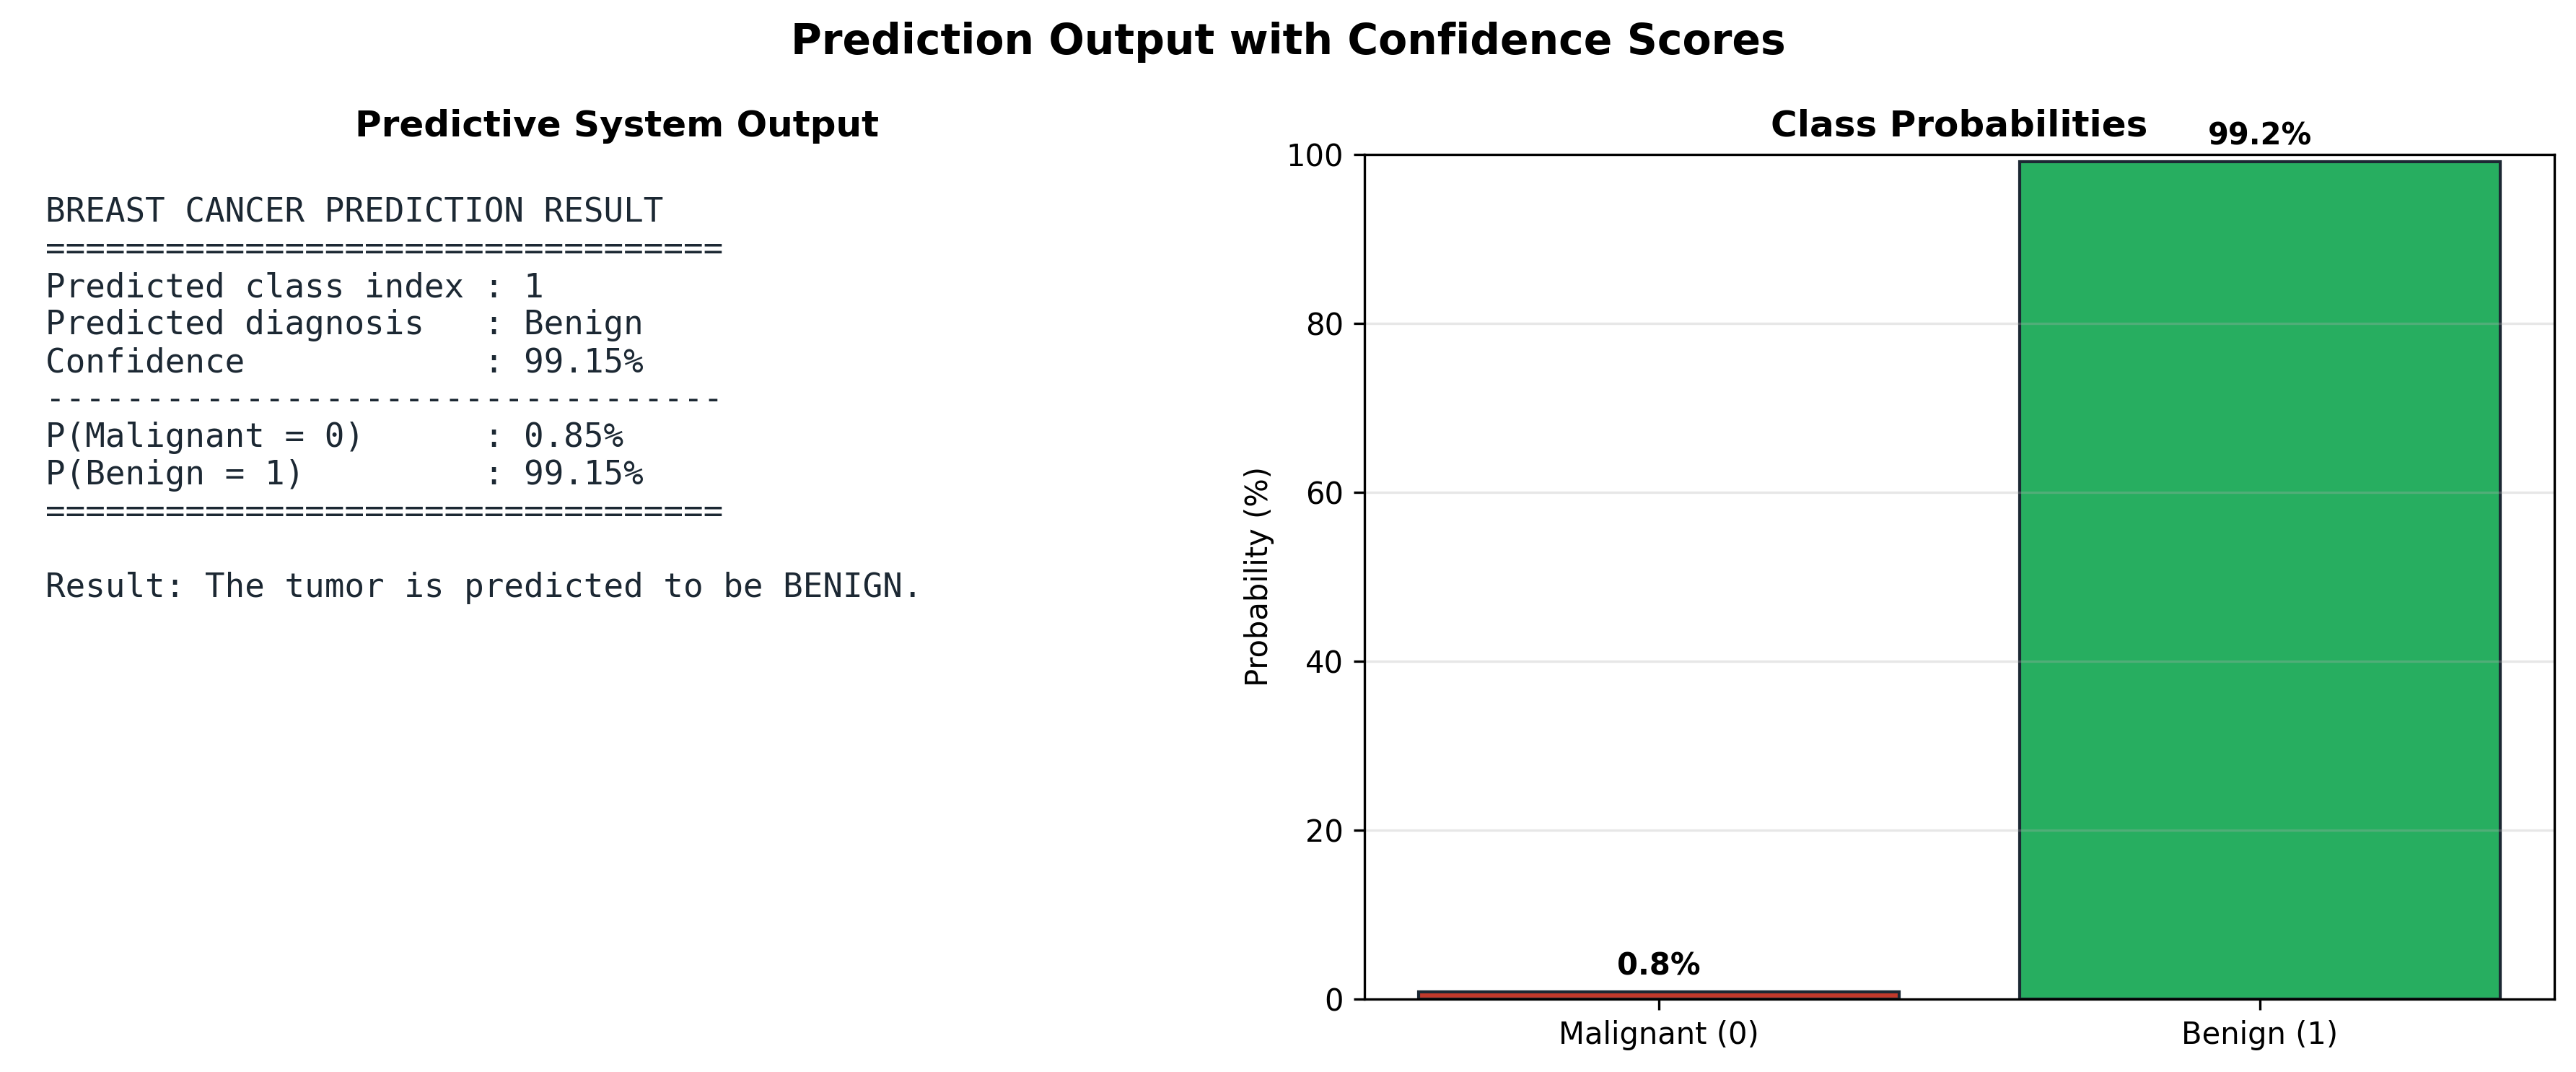
\includegraphics[width=0.92\textwidth,height=0.7\textheight,keepaspectratio]{10_prediction.png}
  \end{center}
\end{frame}

\section{Workflow}
\begin{frame}{Project Workflow}
  \begin{center}
    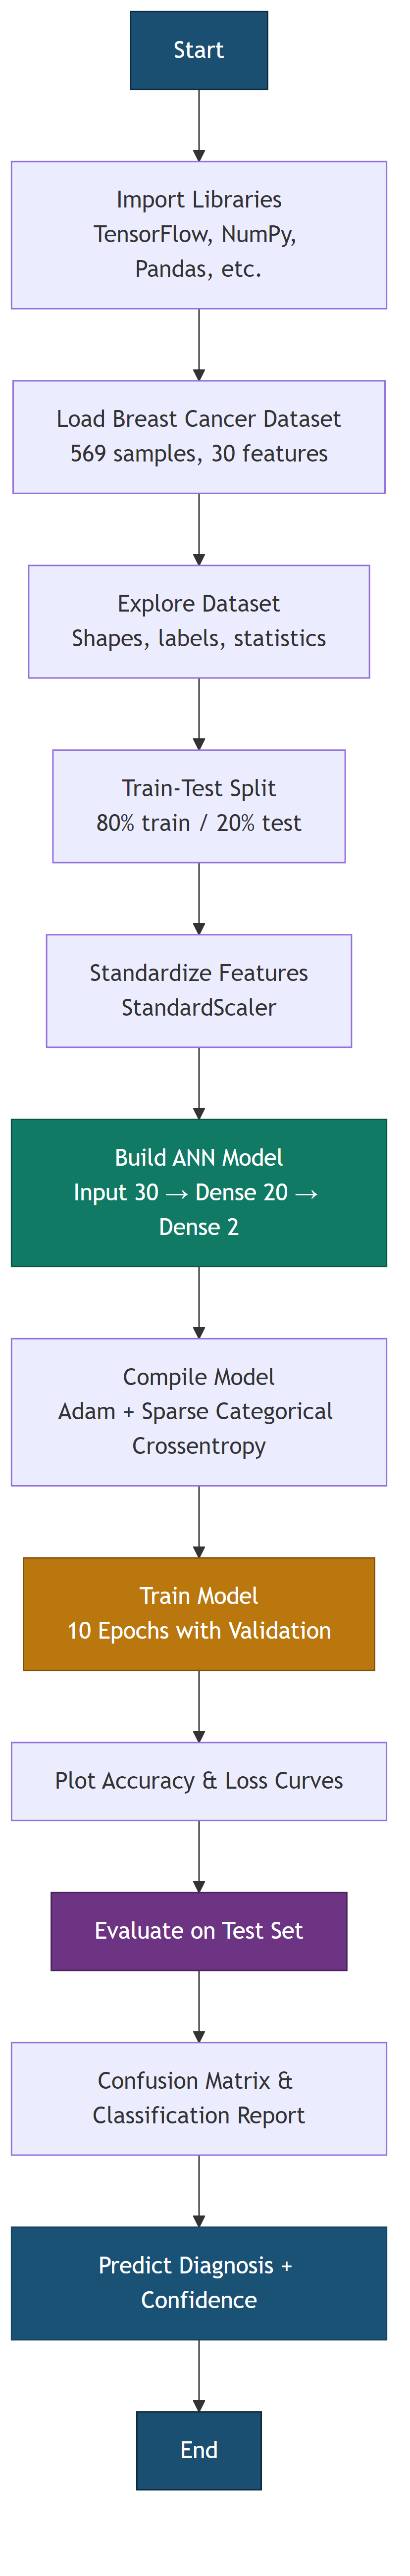
\includegraphics[width=0.45\textwidth,height=0.75\textheight,keepaspectratio]{11_workflow.png}
  \end{center}
\end{frame}

\begin{frame}{Conclusion}
  \begin{itemize}
    \item Built a compact ANN for binary breast cancer classification
    \item Applied stratified split and feature standardization
    \item Evaluated with accuracy, confusion matrix, and classification report
    \item Demonstrated a confidence-aware predictive system
  \end{itemize}
  \vspace{0.6cm}
  {\small\textit{Educational demo only --- not a medical diagnostic tool.}}
\end{frame}

\begin{frame}
  \begin{center}
    {\LARGE Thank You}\\[0.8cm]
    {\large Questions?}
  \end{center}
\end{frame}

\end{document}
